%%
% The BIThesis Template for Bachelor Graduation Thesis
%
% 北京理工大学毕业设计(论文)第二章节 —— 使用 XeLaTeX 编译
%
% Copyright 2020-2023 BITNP
%
% This work may be distributed and/or modified under the
% conditions of the LaTeX Project Public License, either version 1.3
% of this license or (at your option) any later version.
% The latest version of this license is in
%   http://www.latex-project.org/lppl.txt
% and version 1.3 or later is part of all distributions of LaTeX
% version 2005/12/01 or later.
%
% This work has the LPPL maintenance status `maintained'.
%
% The Current Maintainer of this work is Feng Kaiyu.
%%

\chapter{从以太坊到Substrate——使用Rust重构树状区块链}

本章首先分析Substrate开发框架的节点架构,其次介绍官方提供的节点模板,演示在其上进行开发的方法,最后在节点模板的基础上,引入树状区块链的部分特性——账号地理位置,以证明将树状区块链从以太坊开发平台迁移至Substrate开发框架的可行性。

\section{选择Rust的原因}

\secttion{树状区块链实现简析}



树状区块链是在以太坊官方客户端Go-Ethereum的源代码上修改而来,因此,虽然在结构上做出了很大的调整,它也继承了许多Go-Ethereum的特点,例如共识算法和EVM虚拟机等,其性能表现也依然受制于Go-Ethereum。从整体上评估,第三章的3.5.2.1节通过统计学方法,验证了以太坊顺序串行执行交易的特点,这样的执行策略使得以太坊在面对高并发请求时的处理效率不尽如人意;从局部评估,研究\cite{privateChainConsensus}表明,以太坊所使用的共识算法之一——基于工作量的证明(Proof of Work),其性能表现已落后其他更先进的算法。然而,以太坊并未在源代码层面留有太多的可扩展空间,这也意味着许多诸如更换共识算法,修改交易执行逻辑等的自定义修改在实践时困难重重,限制了在以太坊平台改良优化的空间。

Substrate\cite{substrateHome}由Parity Technologies推出,是一套基于Rust编程语言开发的开源的区块链开发框架,允许开发者针对不同的用途对链进行不同程度的定制。在Substrate诞生前,人们花费了大量的精力,试图设计一个支持多链结构的新型区块链。然而,所有这些花费的时间、金钱和精力最终导向了一个结论:当下做出的深思熟虑的选择很可能成为未来的绊脚石。这是因为随着时间的推移,区块链依赖的某些特定的技术或假设,可能会阻碍并最终扼杀创新\cite{substrateDoc}。因此,以太坊创始人之一Gavin Wood成立了Parity技术公司,力图改写这一局面。他们的处女座——以太坊客户端Parity,在相同的硬件配置环境下展现出了远胜Go-Ethereum的性能表现,提升幅度达到了可观的89.8\%\cite{parityVSgeth};在后续开发Parity自研的区块链Polkadot时,Gavin意识到,仅需将Polkadot进行抽象,剥离部分细节,即能获得一个可扩展性极强,适用范围更广的区块链框架。在2018年,Polkadot和用于开发它的区块链框架终于被分离开,成为两个独立的项目,而后者,即是本章讨论的主角——Substrate。

Substrate在设计时,严格遵循三点原则:

\begin{itemize}
    \item 将Rust编程语言作为代码库的核心编程语言。虽然Rust语言的学习曲线较为陡峭,但其极快的速度,极具辨识度的内存管理方式,灵活的抽象能力,以及可编译为WebAssembly的特点使它成为需要高性能表现,强内存安全性,及嵌入式设备友好性等特性之应用场景的不二之选;
    \item 将WebAssembly作为应用程序逻辑的执行环境。WebAssembly是一种新型代码,由万维网联盟创建,可从Rust、C、C++等语言编译获得,且受到多种JavaScript引擎的广泛支持,具有良好的兼容性\cite{wasmIntro}。Substrate的易升级性也建立于WebAssembly的基础之上:它将区块链的具体业务逻辑编译为WebAssembly字节码,并存储于区块链的数据存储区中,用户可以像发起普通交易一样发起一个申请修改链上存储的WebAssembly字节码的交易,从而便利地更新升级区块链系统;
    \item 广泛使用分层抽象、泛型实现和灵活的API作为主要的编码实践,并将库分离为不同的体系结构组件。在核心功能方面,Substrate官方提供了许多不同的实现,例如数据库层的RocksDB和ParityDB,共识层的AURA引擎和Grandpa引擎等,可以任由开发者选择;在应用功能方面,Substrate允许开发者调用官方已开发妥当的模块pallet为他们的区块链添加自定义功能,例如保存并处理账号信息的balances模块,和管理智能合约的contracts模块;不仅如此,Substrate也提供了这些模块的实现源代码,开发者可以自行下载并进行修改后引入区块链,实现功能的定制化。这一设计原则,赋予了Substrate极好的可扩展性,便于开发人员依据实际需要进行功能增删和优化改进等操作。
\end{itemize}

综合以上事实,将树状区块链自以太坊开发平台迁移至Substrate开发框架内,不仅能降低开发难度,获得更好的性能表现和安全性,还能获得更好的兼容性,令区块链能够在浏览器中乃至嵌入式设备上运行,拓宽树状区块链的应用范围。

\section{Substrate节点架构}

在一个去中心化的区块链网络中,每一个节点都同时充当了客户端和服务器的作用,因为它既可以从网络中请求数据,也可以向网络提供数据。Substrate沿用了这一思想,并将其贯彻到了架构设计中。

\begin{figure}[htbp]
    \centering
    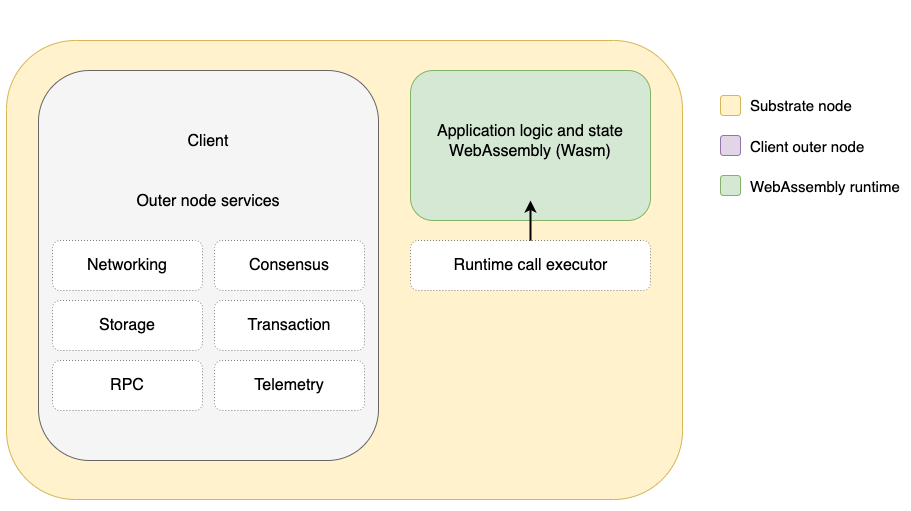
\includegraphics[width=\textwidth]{images/simplified-architecture.png}
    \caption{Substrate节点架构简图}\label{Substrate节点架构简图} % label 用来在文中索引
\end{figure}

如图5-1所示,Substrate节点可以认为由两个部分组成:客户端外部节点以及WebAssembly运行时环境。

\subsection{客户端外部节点}

客户端外部节点负责运行时外部发生的活动。例如,外部节点负责发现对等节点、管理交易池、与其他节点通信以达成共识,以及响应来自外部的RPC调用或浏览器请求。

外层节点处理的一些最重要的活动包括以下几种:

\begin{itemize}
    \item 存储: 使用简单高效的键值对存储层,保存Substrate区块链不断变化的状态;
    \item 点对点网络: 使用libp2p等方式与其他的网络参与者通信;
    \item 共识: 与其他网络参与者通信,确保他们对区块链的状态达成共识;
    \item RPC API:接收入站的HTTP和WebSocket请求,以便区块链用户与网络交互;
    \item 维护节点度量: 通过内嵌的Prometheus服务器收集并提供节点度量相关的信息;
    \item 执行环境: 为运行时选择要使用的执行环境(浏览器中的WebAssembly或本地的Rust环境)然后将调用分派给所选的环境。
\end{itemize}

执行这些任务通常需要外部节点查询运行时以获取信息或向运行时提供信息。这种通信通过调用专门的runtime APIs来处理。

\subsection{WebAssembly运行时环境}

WebAssembly运行时环境确定交易是否有效,并负责处理区块链的状态转换函数的更改。因为运行时能执行它接收到的函数,所以它可以控制如何将交易包含在区块中,以及如何将区块返回到外部节点以传播或导入到其他节点。本质上,运行时负责处理区块链上发生的所有事情,它也是构建Substrate区块链节点的核心组件。

与外部节点向运行时提供信息的方式类似,运行时使用专门的host function与外部通信。

\section{Substrate节点模板介绍}

Substrate官方提供了一份开源的节点模板\footnote{\url{https://github.com/substrate-developer-hub/substrate-node-template}}。节点模板中已包含较完整的运行时环境,且允许开发者自由增删模块,实现功能定制。此外,Substrate也提供了教程文档\footnote{\url{https://docs.substrate.io/tutorials/}},辅助开发者学习使用节点模板。本节将演示在Linux环境下编译节点模板、与节点模板交互、以及为节点模板引入新模块的方法。

\subsection{环境配置}

本章的所有工作在表5-1所示的环境中进行。为提高开发效率,笔者继续使用第四章中搭建的WSL 2环境进行本章的工作。

\begin{table}[htbp]
    \linespread{1.5}
    \zihao{5}
    \centering
    \caption{Substrate相关工作环境}\label{Substrate相关工作环境}
    \begin{tabular}{r|l} \toprule
        中央处理器 & Intel Core i5-12500H      \\
        图形处理器 & Intel Iris Xe 80EU        \\
        内存    & 24GB                      \\
        操作系统  & Ubuntu 22.04.2 LTS        \\
        虚拟机   & Windows Subsystem Linux 2 \\
        \bottomrule
    \end{tabular}
\end{table}

同时,使用节点模板要求安装git、make、clang、curl并配置Rust开发环境\footnote{\url{https://docs.substrate.io/install/linux/}}。

使用如下指令安装包含git、make、clang、curl工具包:

\begin{lstlisting}[caption={安装工具包}, label={lst:安装工具包}]
sudo apt install build-essential
\end{lstlisting}

使用如下指令安装Rust工具链:

\begin{lstlisting}[caption={安装Rust工具链}, label={lst:安装Rust工具链}]
sudo apt install --assume-yes git clang curl libssl-dev protobuf-compiler
curl --proto '=https' --tlsv1.2 -sSf https://sh.rustup.rs | sh
source \$HOME/.cargo/env  # 刷新环境变量

rustup default stable
rustup update  # 更新rust版本为最新的稳定版

# 安装rust nightly的2023-03-21前发布的最新版
rustup update nightly-2023-03-21
rustup target add wasm32-unknown-unknown --toolchain nightly-2023-03-21
\end{lstlisting}

\subsection{使用节点模板进行开发}

本小节主要讨论编译节点模板,及使用Web UI与其交互的方法。

下载节点模板源代码后,观察\verb|runtime/Cargo.toml|。该文件记录了节点模板使用的运行时环境的各项配置。在\verb|dependencies|字段下,写有该运行时包含的各项模块名,及其版本、源代码来源等信息。关于增添新模块和修改官方提供的模块的方法,请见下一小节的介绍。

在源代码根目录中打开终端,执行\verb|cargo build --release|命令,稍事等待至编译完成后,在终端运行\verb|./target/release/node-template --dev|,即能在开发模式下启动节点模板编译而成的节点。

使用Polkadot JS APP连接到该区块链\footnote{\url{https://polkadot.js.org/apps/?rpc=ws\%3A\%2F\%2F127.0.0.1\%3A9944\#/explorer}},在页面导航栏中依次选择“账户” - “账户”,既能看到节点中预定义的账户的各项信息。在导航栏中依次选择“开发者” - “交易”,既能利用WebAssembly运行时环境中引入的模块进行各项操作。如图5-2所示,选择ALICE账户后,依次选择balances模块,选择transfer方法,在Id: AccoundId处选择FERDIE,value处填写10,随后点击“提交交易” - “签名并提交”,即可提交一个转账交易,将10单位代币从ALICE账号余额中转移到FERDIE账号余额中。

\begin{figure}[htbp]
    \centering
    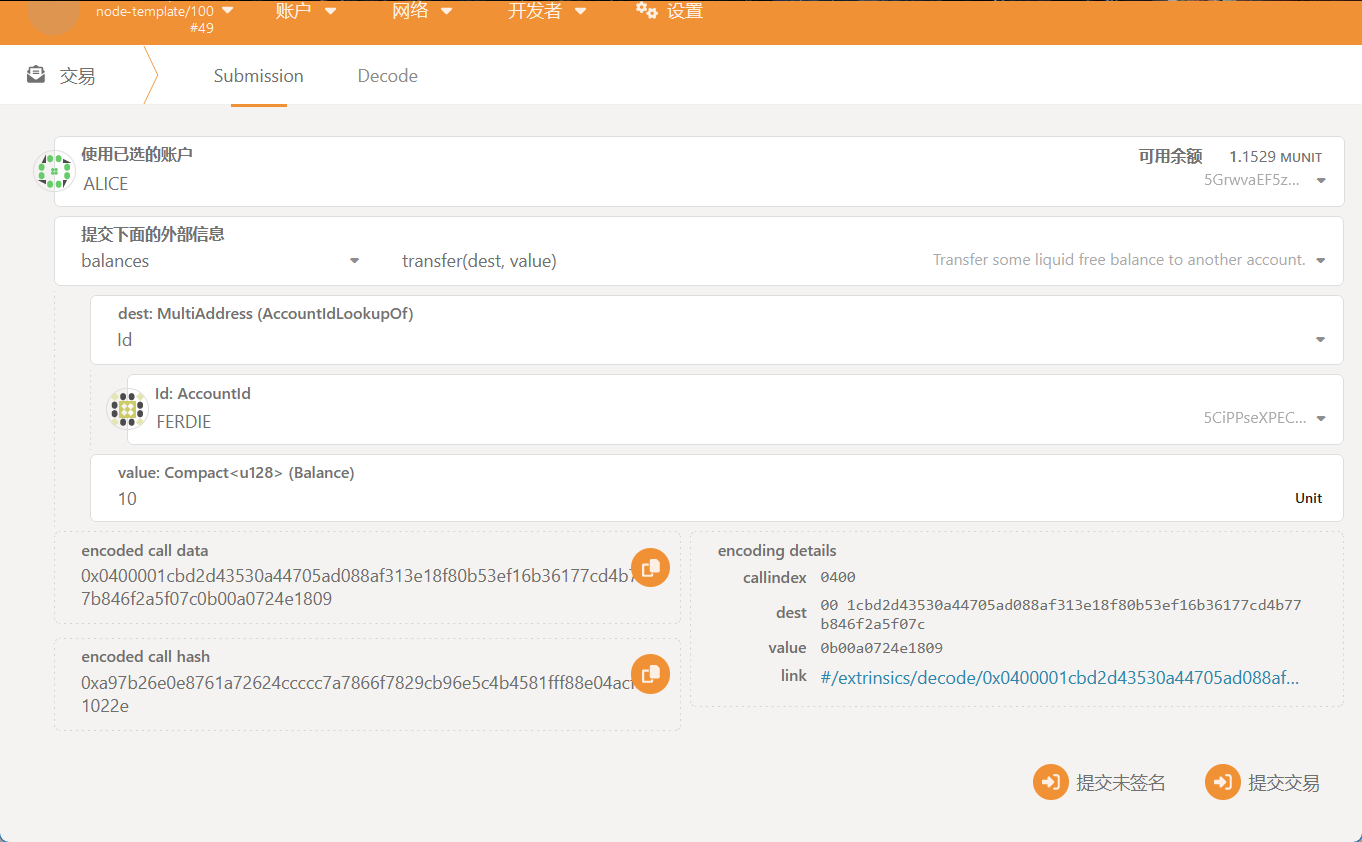
\includegraphics[width=\textwidth]{images/substrateTransfer.png}
    \caption{转账交易示例}\label{转账交易示例} % label 用来在文中索引
\end{figure}

\section{为账户加入地理位置属性}

树状区块链中,为记录每个账号所处的地理位置,向账号结构中加入了地理位置这一字段,以字符串形式存储账号的Geohash编码。本小结将演示如何在Substrate节点模板上实现该效果。

\subsection{更改balances模块的引用源}

模块balances负责记录账号信息,并提供转账等与账号信息有关的功能。为实现账户信息的增添,必须对Substrate官方实现的balances模块源代码进行一定修改。

访问substrate代码仓库\footnote{\url{https://github.com/Endericedragon/substrate/tree/polkadot-v0.9.40}},切换至\verb|polkadot-0.9.40|分支以和节点模板使用的模块所处的分支一致。下载该分支的源代码并将\verb|frame/balances|目录复制到节点模板的\verb|pallets|目录中。

由于下载获得的balances模块源代码使用相对路径引用其他模块,但节点模板目录中并不存在这些路径,故需要将\verb|pallets/balances/Cargo.toml|配置文件中对其他模块的引用修改为从Github上直接引用。举例而言,对于该相对路径引用:

\begin{lstlisting}
sp-std = { version = "5.0.0", default-features = false, path = "../../primitives/std" }

\end{lstlisting}

修改为从Github上直接引用:

\begin{lstlisting}
sp-std = { version = "5.0.0", default-features = false, git = "https://github.com/paritytech/substrate.git", branch = "polkadot-v0.9.40" }
\end{lstlisting}

将所有模块的引用源更改完毕后,保存并关闭\verb|pallets/balances/Cargo.toml|,打开\verb|runtime/Cargo.toml|,将其中对模块\verb|pallet_balances|的引用从Github上引用改为从本地的\verb|pallets/balances|路径引用,修改方法与前文之所述类似,此处不再赘述。

最后,修改节点模板根目录中的\verb|Cargo.toml|:

\begin{lstlisting}
[workspace]
members = [
    "node",
    "pallets/template",
    "pallets/balances",  # <-- 新增这行
    "runtime",
]
[profile.release]
panic = "unwind"
\end{lstlisting}

保存并关闭即可。

\subsection{修改balances模块的源代码}

定义“账户”这一概念的结构体是位于pallets/balances/src/lib.rs源代码的AccountData结构体。笔者在这个结构体中,加入了一个position字段,其类型为笔者自定义的GeoHash类型。增添的代码如下:

\begin{lstlisting}[caption={为balances模块新增代码}]
const GEOHASH_LENGTH: usize = 14;

#[derive(Encode, Decode, Clone, PartialEq, Eq, RuntimeDebug, MaxEncodedLen, TypeInfo)]
pub struct Geohash([u8; GEOHASH_LENGTH]);
impl Default for Geohash {
	fn default() -> Self {
		Geohash([0; GEOHASH_LENGTH])
	}
}
impl Geohash {
	pub fn from(geohash: Vec<u8>) -> Self {
		assert!(geohash.len() <= GEOHASH_LENGTH);
		let mut position: [u8; GEOHASH_LENGTH] = [0; GEOHASH_LENGTH];
		for (i, cc) in geohash.iter().enumerate() {
			position[i] = *cc;
		}
		Geohash(position)
	}
}

// -- snip --

pub struct AccountData<Balance> {
    // --snip --

	// The position of this account, encoded in geohash
	pub position: Geohash,
}
\end{lstlisting}

每个模块均可包含一些方法,开发者可调用这些方法修改链上存储的数据,与模块交互。本小节为balances模块新增两个方法:\verb|set_position()|方法和\verb|transfer_with_position()|方法。

首先,为balances模块新增一个\verb|set_position()|方法,允许账户为自己设置地理位置:

\begin{lstlisting}
#[pallet::call]  // <-- 在pallets/balances/src/lib.rs中全局搜索这行即可找到
impl<T: Config<I>, I: 'static> Pallet<T, I> {
    // -- snip --

    // Set position for oneself
    #[pallet::call_index(6)]
    #[pallet::weight(0)]
    pub fn set_position(origin: OriginFor<T>, new_position: Vec<u8>) -> DispatchResult {
        let sender = ensure_signed(origin)?;
        Self::try_mutate_account(
            &sender,
            |target, _| {
                target.position = Geohash::from(new_position);
                Ok(())
            }
        )
    }
}
\end{lstlisting}

其次,添加一个\verb|transfer_with_position()|方法,令转账发起人提供自身位置信息,用以更新它的\verb|position|字段:

\begin{lstlisting}
#[pallet::call_index(7)]
#[pallet::weight(T::WeightInfo::transfer())]
pub fn transfer_with_position(
    origin: OriginFor<T>,
    dest: AccountIdLookupOf<T>,
    #[pallet::compact] value: T::Balance,
    position: Vec<u8>
) -> DispatchResultWithPostInfo {
    let transactor = ensure_signed(origin)?;
    let dest = T::Lookup::lookup(dest)?;
    <Self as Currency<_>>::transfer(
        &transactor,
        &dest,
        value,
        ExistenceRequirement::AllowDeath,
    )?;
    Self::try_mutate_account(
        &transactor,
        |target, _| {
            target.position = Geohash::from(position);
            Ok(().into())
        }
    )
}
\end{lstlisting}

至此,对代码的修改暂告一段落。以上修改已形成文档\footnote{\url{https://github.com/Endericedragon/substrate-node-template/blob/main/\%E4\%BF\%AE\%E6\%94\%B9\%E8\%AE\%B0\%E5\%BD\%95.md}},以便后人阅读参考。

\subsection{编译并测试修改结果}

在节点模板根目录中运行\verb|cargo build --release|命令进行编译,确认编译过程无任何错误并结束后,使用5.3节的方法启动测试链并将Web UI连接至测试链上。在导航栏上点击“开发者” - “交易”,选择ALICE账号并按图5-3所示填写交易的各项参数,以调用balances模块的\verb|set_position()|方法。提交设置位置的交易图中的wx4111b即为目标账户新地理位置的Geohash编码。需要注意的是,5.3.2小节的代码中设置了该字段的限长\verb|GEOHASH_LENGTH|为14,故提交的字符串长度必须小于该限长。

\begin{figure}[htbp]
    \centering
    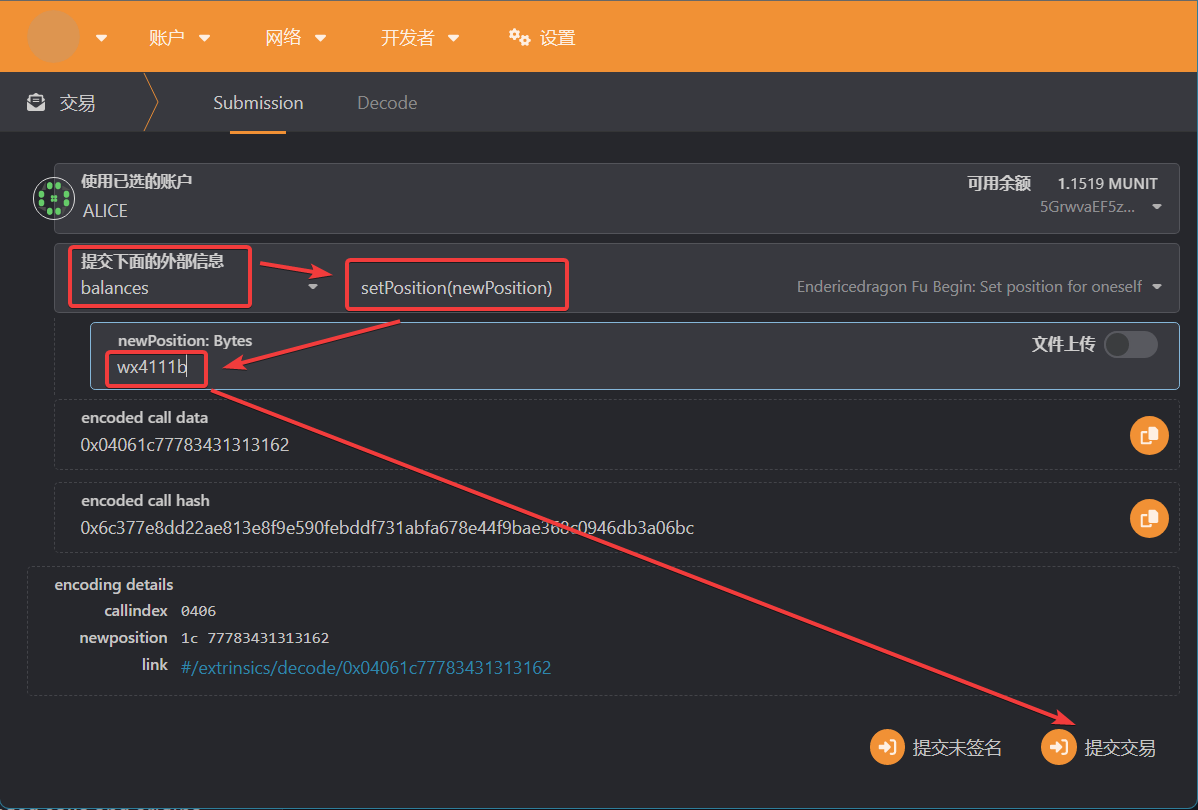
\includegraphics[width=\textwidth]{images/setPos.png}
    \caption{发起设置位置交易}\label{发起设置位置交易} % label 用来在文中索引
\end{figure}

待签名并提交该交易后,点击导航栏上的“开发者” - “链状态”,按图5-4所示填写查询信息。点击界面右侧的加号,查询结果将立刻显示在界面下方,可以看到账户信息中出现了position字段,其值为0x7778343131316200000000000000。此即为提交的字符串的16进制编码,按照两位16进制编码对应一个ASCII字符的规则进行转码后,还原其记录的字符串信息即为\verb|wx4111b|,与上一步骤中提交的交易参数一致。

\begin{figure}[htbp]
    \centering
    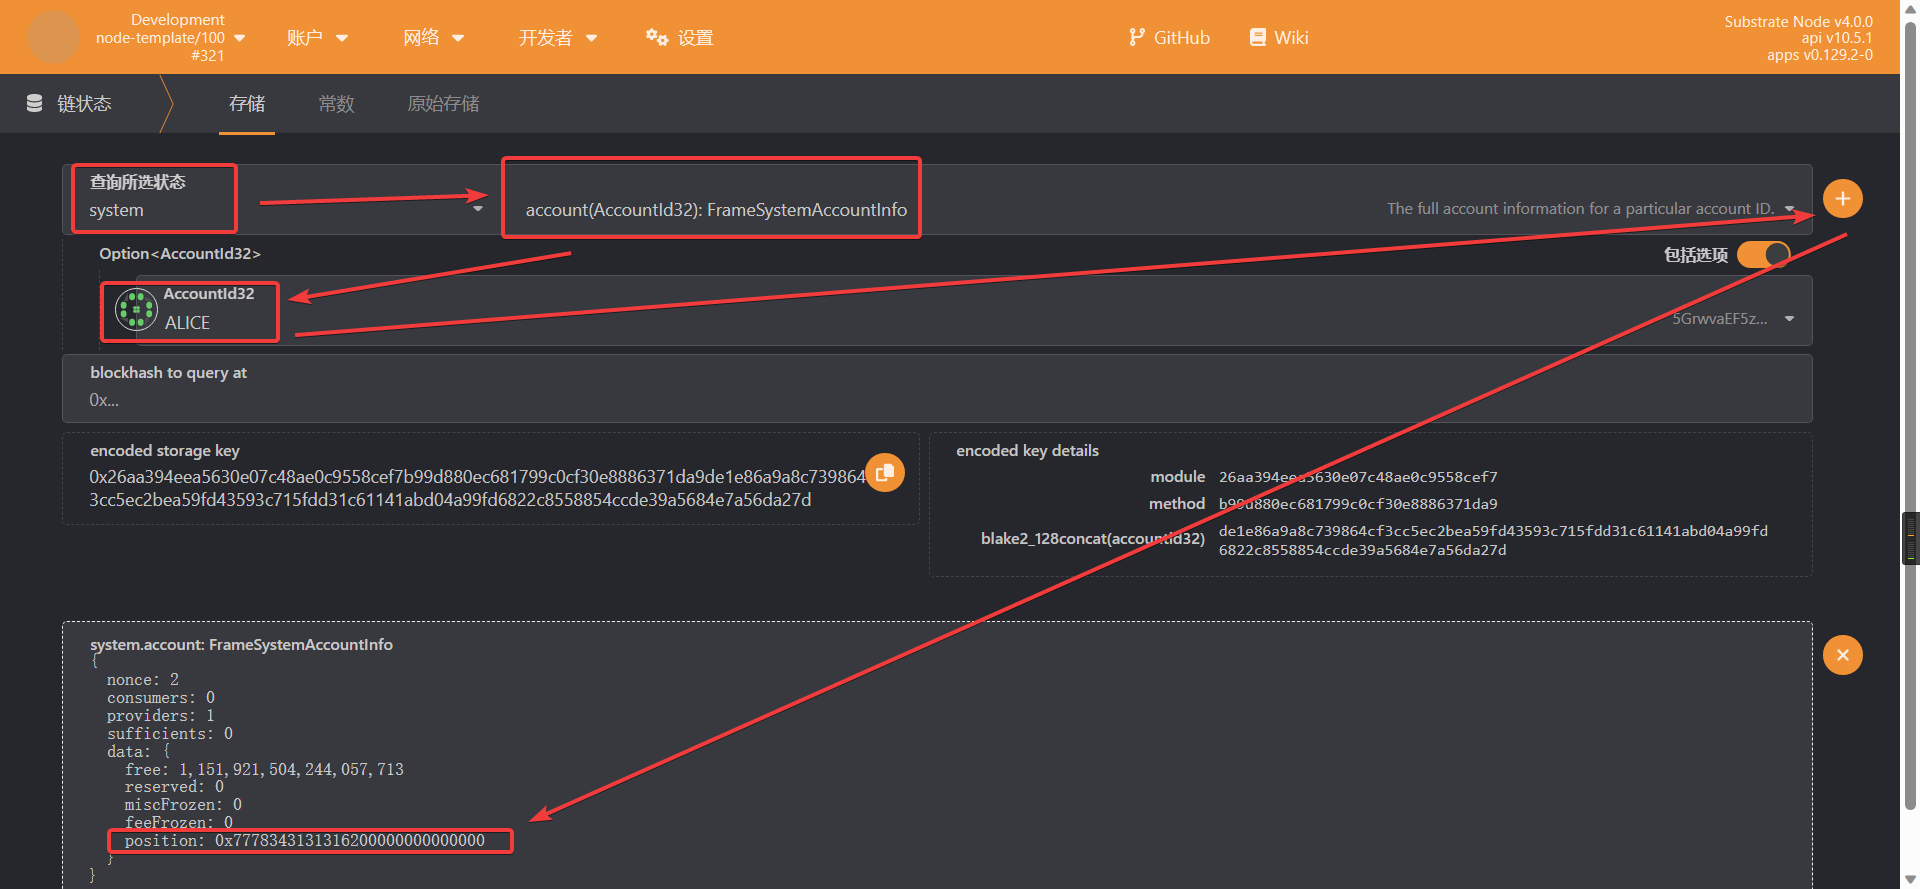
\includegraphics[width=\textwidth]{images/watchAccInfo.png}
    \caption{查询账户信息}\label{查询账户信息} % label 用来在文中索引
\end{figure}

使用相似的方法,调用balances模块的\verb|transfer_with_position()|方法,令账号ALICE在wx4111c位置处发起转账,如图5-5所示。

\begin{figure}[htbp]
    \centering
    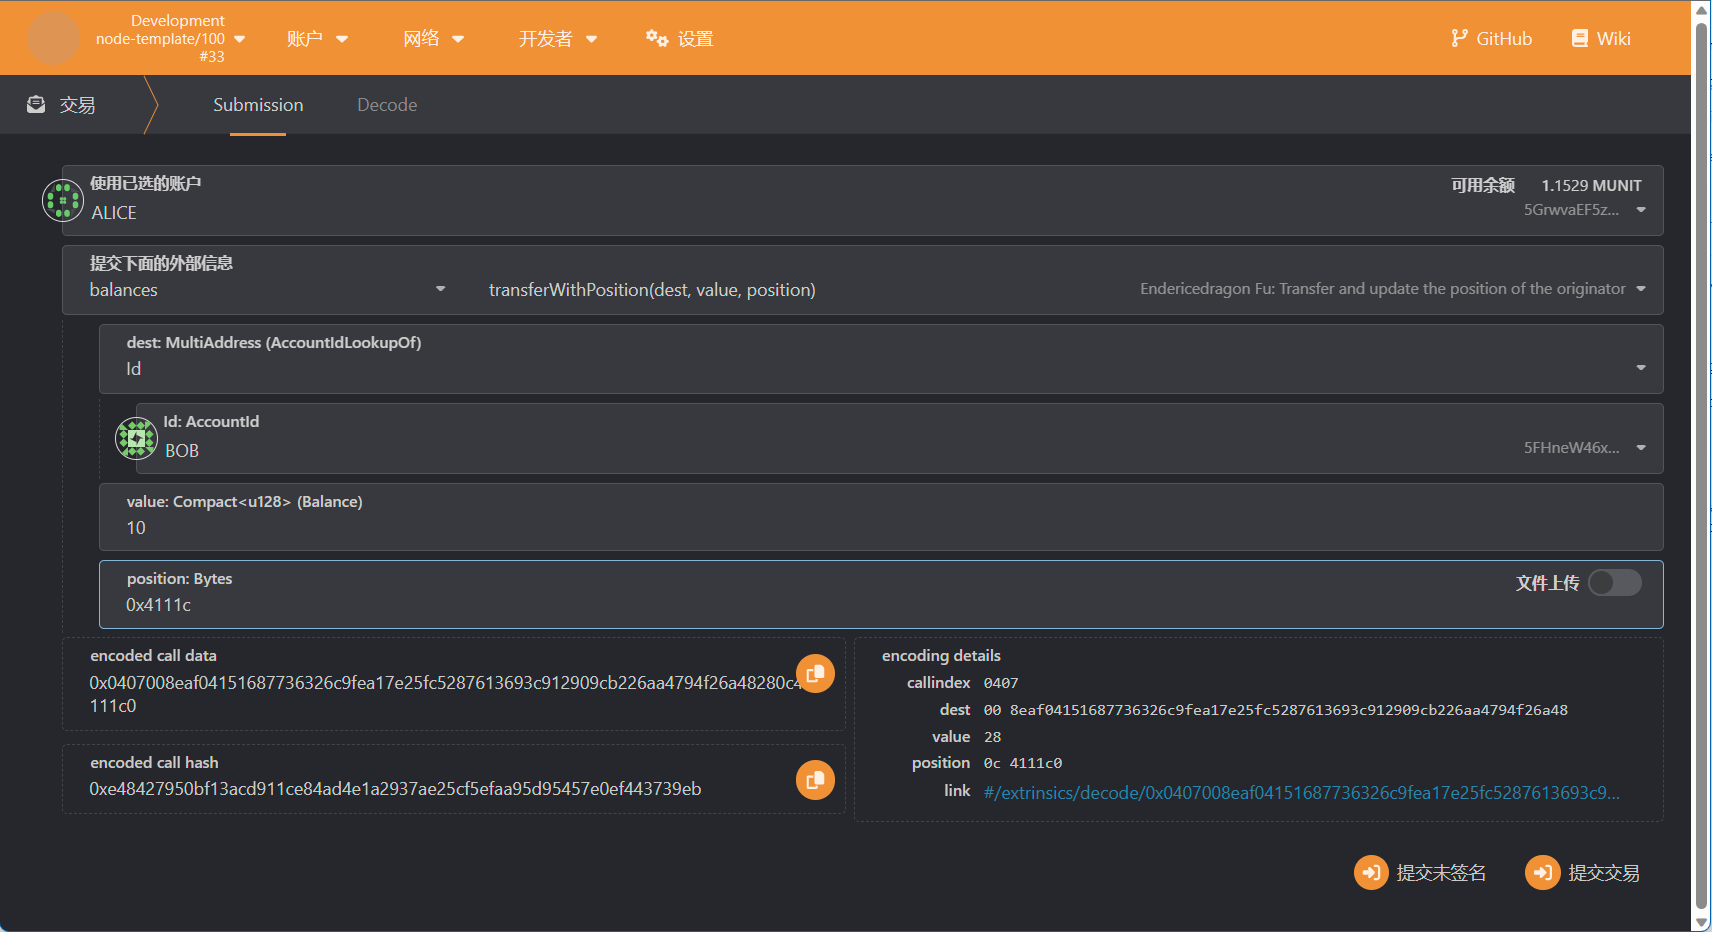
\includegraphics[width=\textwidth]{images/transWithPos.png}
    \caption{调用带位置信息的转账方法}\label{调用带位置信息的转账方法} % label 用来在文中索引
\end{figure}

随后,查询转账发起人ALICE的位置信息,获得图5-6所示的输出。其中,position字段的值0x77783431313163即为ALICE的新位置Geohash编码wx4111c的16进制表示。

\begin{figure}[htbp]
    \centering
    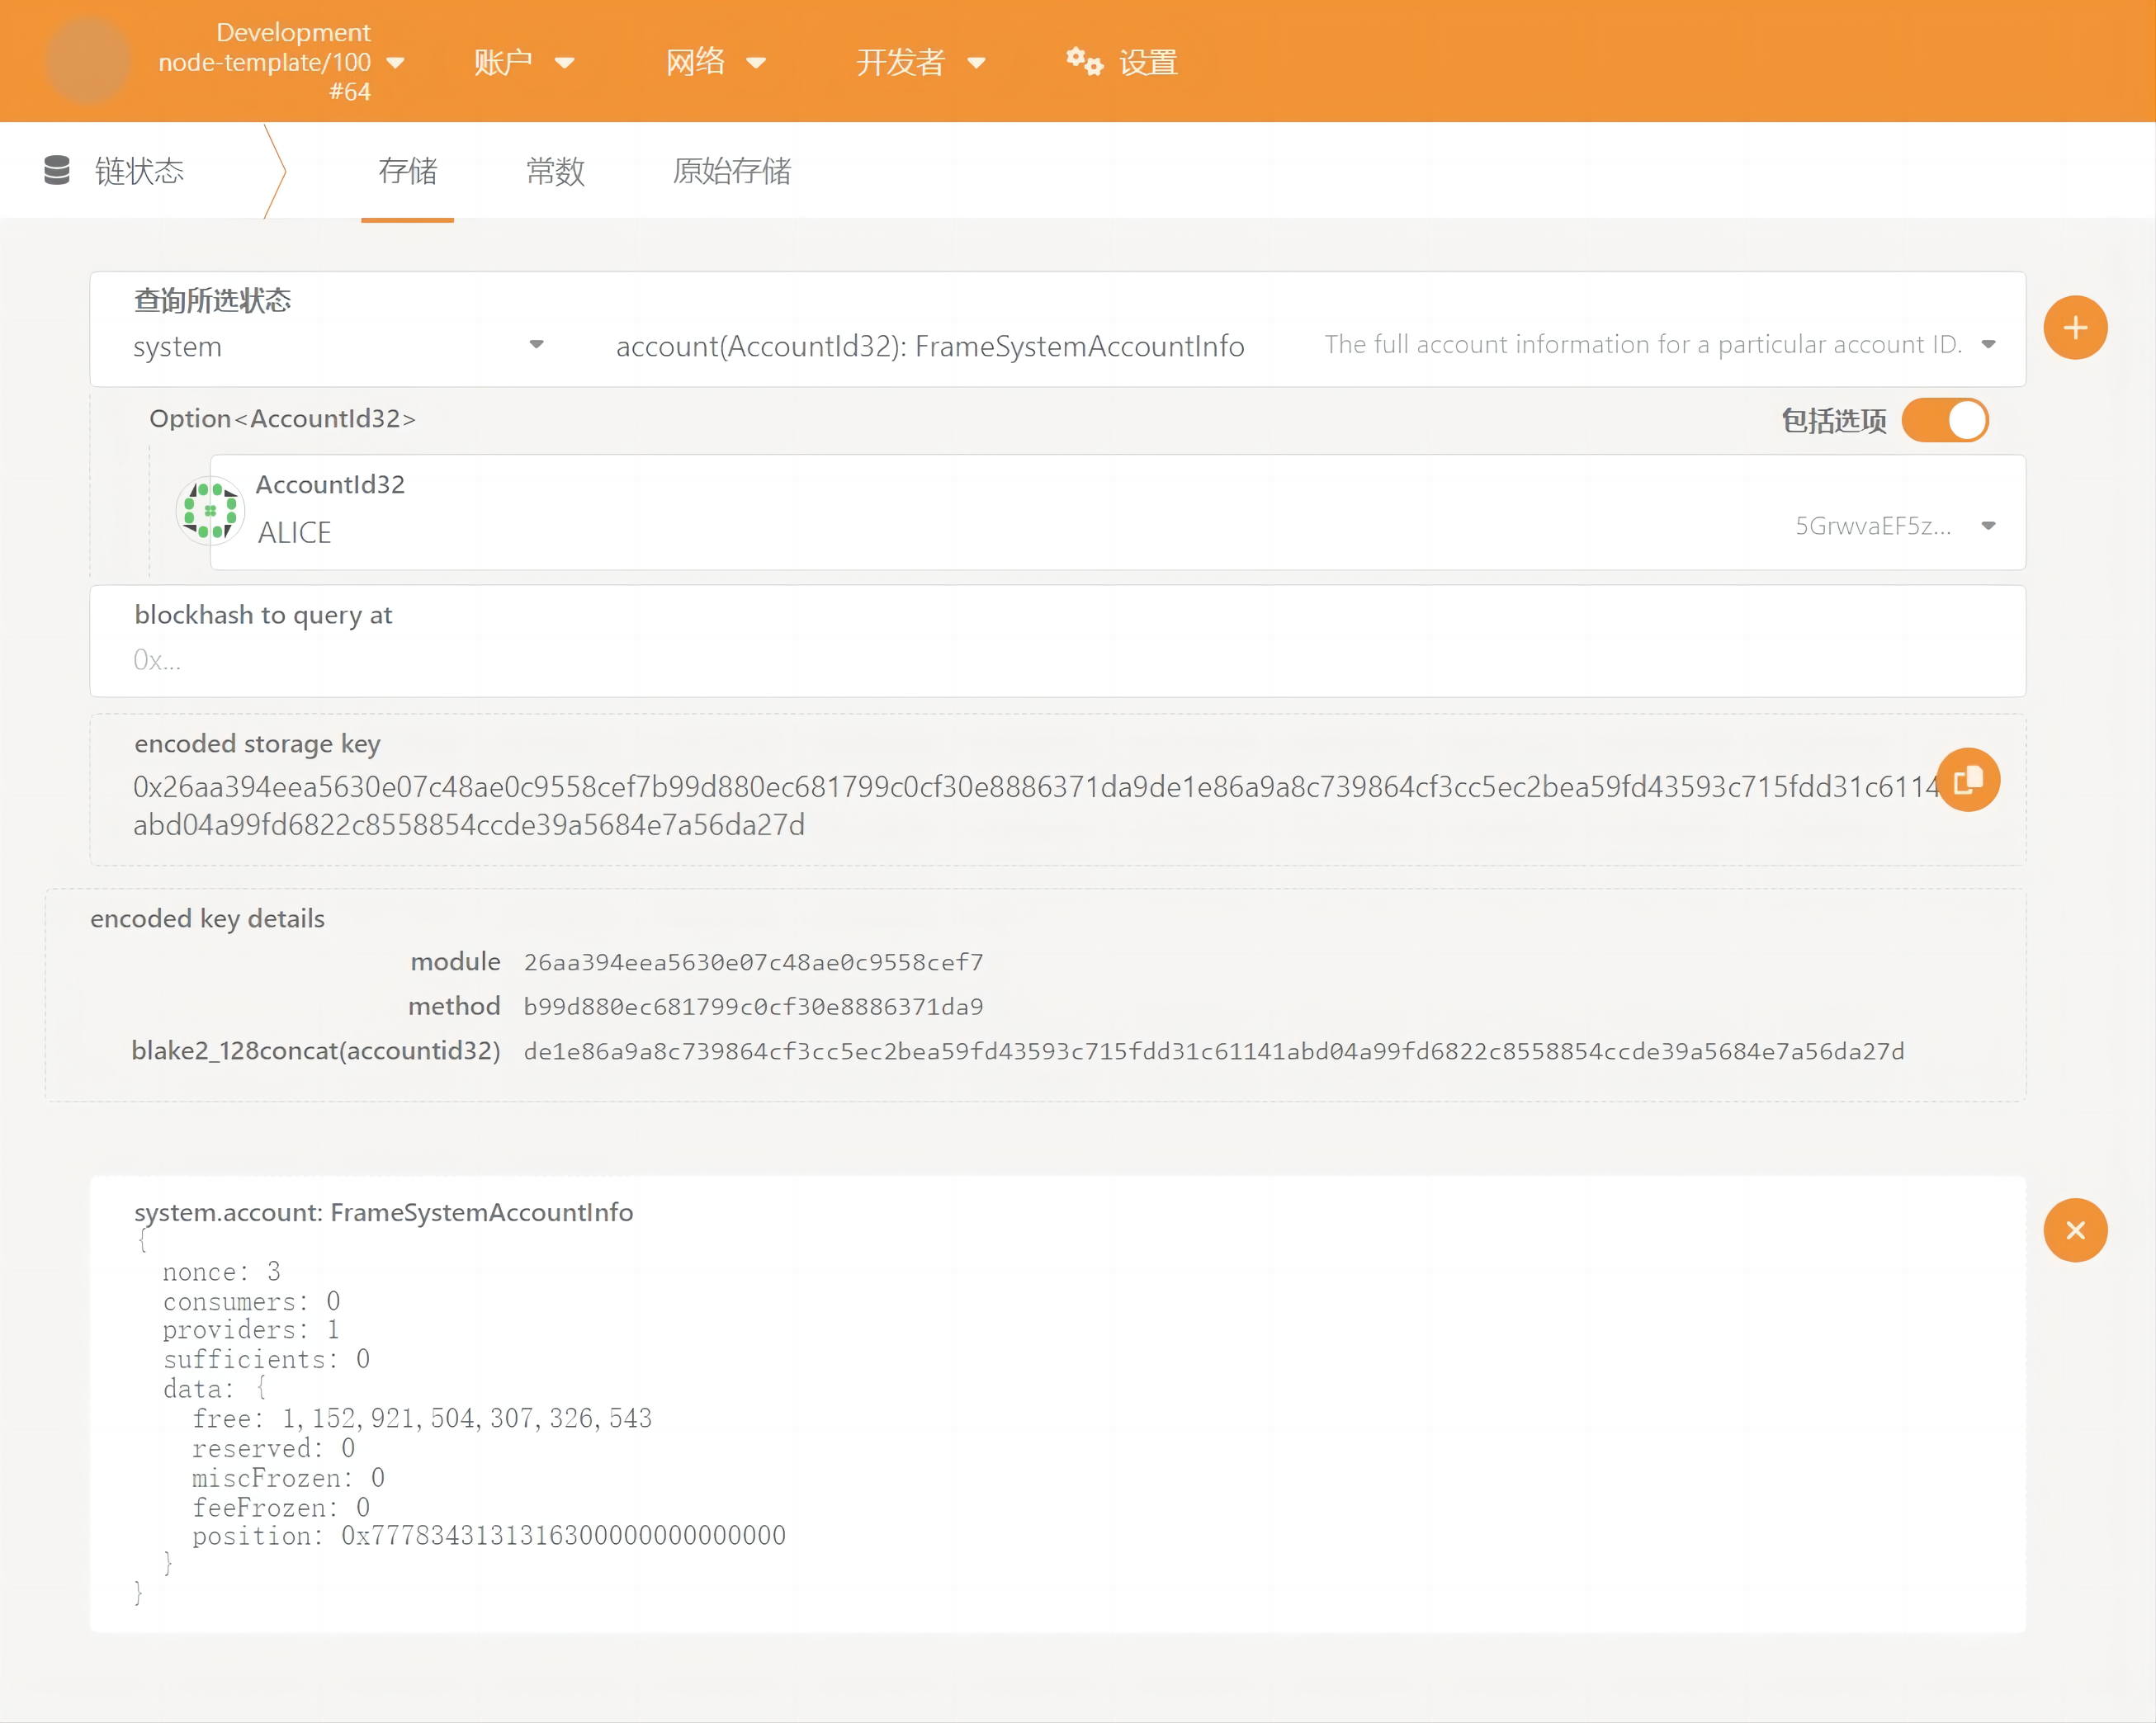
\includegraphics[width=\textwidth]{images/transWithPosResult.png}
    \caption{转账发起人位置已更新}\label{转账发起人位置已更新} % label 用来在文中索引
\end{figure}

至此,账户信息中已包含地理位置字段。通过完成树状区块链部分特性在Substrate框架中的实现,本节工作证明了Substrate具有优秀的可扩展性,也为树状区块链的改进工作指明了方向。

\section{本章小结}

本章首先比较了Substrate相较以太坊的优势并介绍了Substrate的特点,阐述了树状区块链的改进思路,即将其从以太坊平台迁移至扩展性更强,综合性能更佳的Substrate开发框架。其次,介绍了Substrate的节点架构,其可分为客户端外部节点和WebAssembly运行时环境两大板块,分别负责不同类型的事务处理。最后,介绍了使用节点模板进行运行时开发的方法,并成功将树状区块链的部分功能特性迁移到节点模板上,证明了树状区块链改进思路的可行性。
